\documentclass{hitreport}
% =============================================
% Part 0 Edit the info
% =============================================

\major{大数据科学与技术}
\name{冯运}
\title{大数据计算基础}
\stuid{1160300524} % 学号
\date{2019-01-12}
\lab{} %实验地点
\course{商业大数据—电视数据中的群体收视行为计算与挖掘}
\instructor{必修}
\grades{}
\expname{} %实验名称
\exptype{} % 实验类型
\partner{} % 同组学生名字

\begin{document}
% =============================================
% Part 1 Header
% =============================================
\makecover

% =============================================
% Part 2 Main document
% =============================================

\section{问题描述}
题号:06\par
题目名称: \\
商业大数据—电视数据中的群体收视行为计算与挖掘\par
\subsection{题目内容}
应用背景:\\
目前,在商业领域,各类行业机构都已意识到数据的重要性,“数据资产”概念应运而生,而如何运用好多年积累的数据,从而使其在商业决策中发挥更大的价值成为现在的研究热点之一。当今时期,广播电视节目百花齐放,种类繁多,电视用户有了更多的收视选择并可能形成有规律的收视习惯。对于群体性收视行为的计算能够帮助了解用户的收视习惯,对了解民众的生活风貌具有宝贵的社会学价值,对企业的广告投放和节目配比也有重要的商业价值。本实验的研究目标为设计高效的算法,实现对大规模电视数据的用户收视行为特征的计算,结合数据挖掘和逻辑回归分析、相关性分析等统计学方法对该部分数据进行知识挖掘和发现。数据来源某地区一个月的电视用户的收视记录,覆盖用户总人数十万级,记录总量10G.\par
设计部分:\\
充分熟悉数据,首先利用统计学模型对用户的收视时间、收视时长、各类型节目的收视频率进行建模分析,然后对于每个用户设计状态转移图,设计有效的算法,对大量用户的收视喜好等特征进行计算和规律挖掘;并结合实验,对算法进行优化,提高算法的效率。\par
实验部分:\\
应用一种大数据计算系统,实现“设计部分”所要求的算法,利用实验数据,设计对比实 验,采用合适的实验指标,测试本实验提出的算法与已有算法的性能(包括效果、效率)对比结果,并能够对实验结果进行合理分析。

\subsection{问题的技术难点}
\begin{flushleft}
  对原始数据有效信息的解析和提取\\
  数据的管理与统计\\
  对用户收视喜好特征的挖掘
\end{flushleft}

\section{基于的系统与算法}
\begin{flushleft}
  计算系统:
  Spark\\
  \paragraph{系统架构:}
  \begin{flushleft}
    Spark是基于内存计算的大数据并行计算框架.Spark基于内存计算,提高了在大数据环境下数据处理的实时性,同时保证了高容错性和高可伸缩性,允许用户将Spark部署在大量的廉价硬件之上,形成集群\par
    Spark由以下几个部分组成:\\
    Cluster Manager:在standalone模式中即为Master主节点,控制整个集群,监控worker。\\
    Worker节点:从节点,负责控制计算节点,启动Executor或者Driver。\\
    Driver: 运行Application 的main()函数\\
    Executor:执行器,是为某个Application运行在worker node上的一个进程\par
    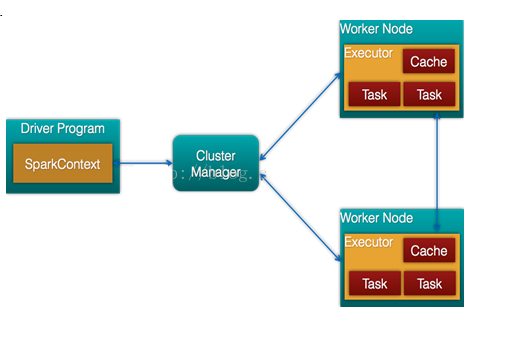
\includegraphics[width=1\linewidth]{frame.png}
    本实验使用的系统有以下几个库:\\
    Spark Core:包含Spark的基本功能;尤其是定义RDD的API、操作以及这两者上的动作。其他Spark的库都是构建在RDD和Spark Core之上的\\
    Spark SQL:提供通过Apache Hive的SQL变体Hive查询语言(HiveQL)与Spark进行交互的API。每个数据库表被当做一个RDD,Spark SQL查询被转换为Spark操作。\\
    MLlib:一个常用机器学习算法库,算法被实现为对RDD的Spark操作。这个库包含可扩展的学习算法,比如分类、回归等需要对大量数据集进行迭代的操作。\\
  \end{flushleft}
  \paragraph{系统优势}
  \begin{flushleft}
    本实验的数据需要使用机器学习的算法进行迭代分析,对效率和性能的要求较高,而Spark是一个内存计算框架,在迭代时使用内存存储中间数据能够有效提高计算效率\\
    此外,Spark支持使用SQL语言对数据进行管理和统计,能够减小实现难度
  \end{flushleft}
  \paragraph{系统使用方法}
  \begin{flushleft}
    我使用了Spark中的Spark Core,Spark SQL, Spark Mllib三个库,Spark Core用来提供基本的RDD数据存储结构,Spark SQL提供数据管理的相关支持,Mllib提供数据挖掘中的算法实现。\\
    通过调用Spark提供的Java API来使用Spark系统,首先读取原始文件存储为RDD格式,然后转换成SparkSQL定义的Dataset格式,使用SQL语句对RDD进行管理和统计,最后调用Mllib中的相关机器学习算法对数据进行模型训练,得到用户收视喜好特征。
  \end{flushleft}

\end{flushleft}

\section{系统与算法设计}
\subsection{系统设计}
\subsubsection{系统组成}
\begin{itemize}
  \item 原始记录解析模块\\
        功能:这个模块负责从原始收视记录中提取有效的数据,存储进RDD中。\\
        实现:构造一个抽象类: Event ,这是对一条用户收视记录的抽象,包括typeID(事件的类型),recordTime(记录产生的时间),CACardID(用户CA卡的卡号)\\
        以下是typeID 与 事件的对应关系\\
        ~\\
        \begin{tabular}{|c|c|}
          \hline
          typeID & 事件类型     \\
          \hline
          1      & 开机事件     \\ \hline
          2      & 关机事件     \\ \hline
          21     & 频道进入事件 \\ \hline
          5      & 频道退出事件 \\ \hline
          23     & 用户喜欢频道 \\ \hline
          97     & 时移节目播放 \\ \hline
        \end{tabular}\\
        ~\\
        事件类型选择的原因:\\
        开机事件和关机事件用来挖掘用户收看节目的时间喜好,
        频道进入退出事件可以用于挖掘用户对不同节目的喜好\\
        由于每种事件包含的信息不同,所以需要不同的子类去继承Event父类\\
        以下是不同的事件类型对应的类名\\
        ~\\
        \begin{tabular}{|c|c|}
          \hline
          ClassName           & 事件类型     \\ \hline
          event               & 抽象时间类型 \\ \hline
          openEvent           & 开机事件     \\ \hline
          closeEvent          & 关机事件     \\ \hline
          channelEvent        & 频道抽象事件 \\ \hline
          channelEnterEvent   & 频道进入事件 \\ \hline
          channelQuitEvent    & 频道退出事件 \\ \hline
          channelCollectEvent & 用户喜欢频道 \\ \hline
          timeShiftShowEvent  & 时移节目播放 \\ \hline
        \end{tabular}\\
        ~\\ \newpage
        类继承关系图:\\
        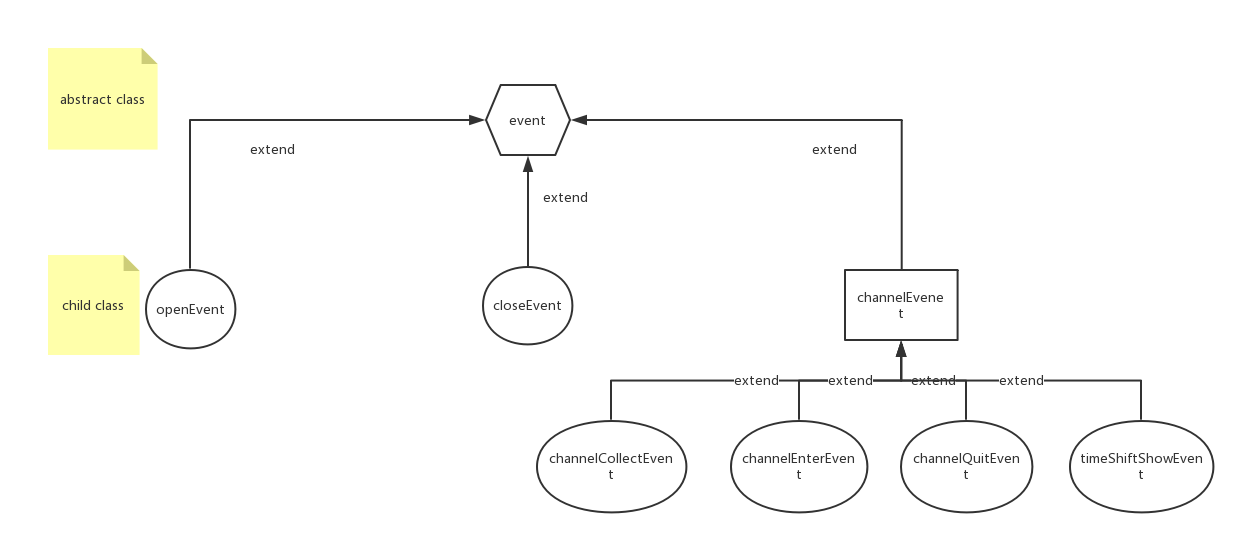
\includegraphics[width=1\linewidth]{class.jpg}\\
        在event类中有一个工厂函数,传入一条原始事件记录的字符串,然后工厂函数使用正则表达式解析出事件类型,然后返回事件对应的对象\\
        这个系统把所有读入原始数据记录并行调用event的工厂函数,然后将得到的对象存储RDD,当所有都进行完成后,将RDD保存成序列化的文件存储在
        系统中,便于之后的数据统计与分析使用,同时避免每次都解析原始数据,从而大幅度提高处理效率。
  \item 数据统计模块\\
        这个模块用于读取数据解析模块得到的事件RDD,使用SpqrkSQL对RDD进行一系列统计分析,得到该地区大体的收视规律\\
        实现:
        \begin{itemize}
          \item 计算收视率: \\
                设计了一个功能API,
                \begin{lstlisting}
              private static void getTVRatings(Dataset<Row> channelEventsDS, Timestamp startTime, Timestamp endTime)
            \end{lstlisting}
                用于计算在某一时间段内所有节目的收视率\\
                收视率计算公式:$$rating = c(show) \div c(all)$$
                c(show)表示收看节目的人数
                计算过程详见算法介绍部分

          \item 计算用户收视时长
                定义了一个计算用户在某一段时间的收视时长的API:
                \begin{lstlisting}
              private static void getWatchTime(Dataset<Row> eventsDS, String CACardID, Timestamp startTime, Timestamp endTime)
            \end{lstlisting}
                API返回用户观看的时长统计,计算过程详见算法部分
          \item 计算收视时间
                定义了一个计算该地区每天不同时间段收看人数的API:
                \begin{lstlisting}
              private static void watchTime(Dataset<Row> eventsDS)
            \end{lstlisting}
                API返回一天24个小时中每个小时段观看电视的人数,计算过程详见算法部分
          \item 用户状态转移图
                定义了一个获得某个用户状态转移图的API:
                \begin{lstlisting}
            private static void getUserStatusTransform(SparkSession sparkSession, String CACardID, Timestamp startTime, Timestamp endTime)
          \end{lstlisting}
                API返回某个用户的收视状态转移图,计算过程详见算法部分
        \end{itemize}
  \item 数据挖掘模块
        \begin{itemize}
          \item 对某个节目收视人数的预测
                实现:
                \begin{enumerate}
                  \item 对全部用户的收视事件进行随机抽样,抽取到1000个节目,按照7:3的比例划分成训练集和测试集。
                  \item 对每个节目构建四个维度的特征向量: 节目开始时间,节目类型,节目所属电视台的影响力权重,以及其实际的收视人数。
                        其中 开始时间,节目类型,节目所属电视台的影响力权重是输入维度,节目实际观看人数是输出维度
                  \item 对得到的训练集使用几种不同的回归模型进行训练,统计算法运行的时间
                  \item 使用测试集作为输入,将模型的预测收视人数和实际收视人数比较,得到误差均值
                  \item 比较几种回归模型的准确率和算法性能,使用准确率和算法性能均衡的算法作为最终的预测模型
                \end{enumerate}
                注: 由于节目所属的类型无法使用程序自动获得,在系统中使用人工标注的方式获得,每种节目类型用一个正整数表示,然后作为一个特征维度
                以下是各种类型节目对应的编号:
                ~\\
                \begin{tabular}{|c|c|}
                  \hline
                  儿童     & 1  \\ \hline
                  综艺     & 2  \\ \hline
                  电视剧   & 3  \\ \hline
                  电影     & 4  \\ \hline
                  体育     & 5  \\ \hline
                  新闻     & 6  \\ \hline
                  法制     & 7  \\ \hline
                  财经     & 8  \\ \hline
                  戏曲     & 9  \\ \hline
                  购物     & 10 \\ \hline
                  纪录片   & 11 \\ \hline
                  科教     & 12 \\ \hline
                  音乐     & 13 \\ \hline
                  军事     & 14 \\ \hline
                  道德文化 & 15 \\ \hline
                \end{tabular}\\
                ~\\
          \item 对某个用户电视节目的推荐
                \begin{enumerate}
                  \item 对全部用户的收视事件进行随机抽样,抽取到1000个样本,按照7:3的比例划分成训练集和测试集。
                  \item 对每个用户构造15个维度的特征向量,维度i代表该用户在节目类型i的收视时间总长
                  \item 使用聚类算法对用户的15个特征进行聚类,得到聚类结果。被聚为一类的用户代表其有相似的收视喜好
                  \item 对一个新用户进行节目推荐时,首先构造其特征向量,然后用聚类模型对其归类,为该用户推荐同类用户喜爱的节目,从而实现推荐功能
                \end{enumerate}
        \end{itemize}
  \item 展示模块\\
        功能: 将系统的统计与挖掘结果进行输出展示\\
        实现: 目前是直接控制台打印输出,后续可以使用图标或者提供web服务的方式对客户进行展示
\end{itemize}
系统架构图:\\
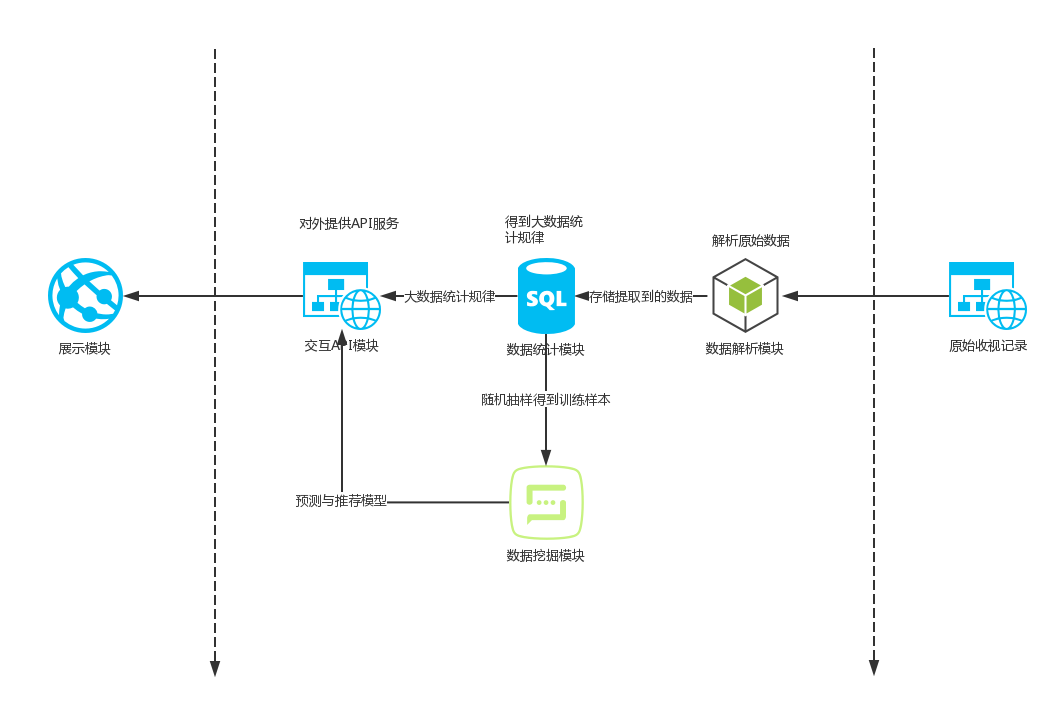
\includegraphics[width=1\linewidth]{structure.png}
\subsection{算法设计}
\begin{itemize}
  \item 收视率计算算法:\\
        input : Dataset<Row> channelEventsDS, Timestamp startTime, Timestamp endTime\\
        output : Dataset<Row> rating\\
        过程:
        \begin{enumerate}
          \item 使用 startTime 和 endTime 对 channelEventsDS 进行筛选
          \item 对CACardId进行去重,只保留一项该ID的记录
          \item 对(2)处理后的数据进行计数求和,得到sum
          \item 将数据对 channel(频道)和show(节目) 两个属性进行group操作,得到每个节目对应的所有观众
          \item 对每个节目的观众数据计数求和,得到sum(i)
          \item 得到节目 i 的收视率: $$rating(i) = sum(i)\div sum \times 100\% $$
        \end{enumerate}
  \item 计算用户收视时长算法: \\
        input : Dataset<Row> eventsDS, String CACardID, Timestamp startTime, Timestamp endTime
        output : Long watchTime // 用户在时间段内的收视时间
        过程:
        \begin{enumerate}
          \item 使用 startTime 和 endTime 对 channelEventsDS 进行筛选
          \item 在所有的数据中筛选出 CACardID == "CACardID"的所有事件
          \item 在(2)中筛选出事件类别为channelQuitEvent的事件
          \item watchTime <- (3)结果中事件的 lastTime 属性值全部相加
        \end{enumerate}
  \item 计算收视时间算法\\
        input: Dataset<Row> eventsDS
        output: List<Long> watchTime
        过程:
        \begin{lstlisting}
          tempDS <- eventDS // 避免后续操作对原始数据的改变
          for h <- 0 to 23 do:
            tempDS <- tempDS.filter(time between h and h+1)
            tempDS <- tempDS 对 CACardID 去重
            watchTime[h] <- tempDS 计数
          end
          return watchTime
        \end{lstlisting}
  \item 用户状态转移图算法\\
        input: SparkSession sparkSession, String CACardID, Timestamp startTime, Timestamp endTime
        output: Dataset<Row> states
        过程:
        \begin{enumerate}
          \item data <- sparkSession.load("file")
          \item 使用 startTime 和 endTime 对 data 进行筛选
          \item 在所有的数据中筛选出 CACardID == "CACardID"的所有事件
          \item 对所有的时间以 recordTime 为基准从早到晚排序,得到states(用户状态的转换)
        \end{enumerate}
  \item 回归模型算法\\
        \begin{itemize}
          \item 线性回归算法:\\
                假设矩阵 X 的每一行表示一个样本,每一列表示相应的特征,列向量 Y 表示矩阵 X 所对应的取值,那么我们需要找到一个列向量 $\Theta$ 使得 $Y=X\Theta$。
                $$\sum_{i=1}^{m}(y_i-x_i\theta)^2 = (Y-X\theta)^T(Y-X\theta)$$
                的取值足够小,对$\theta$求导后,令导数为0,得到$$\theta = (X^TWX)^{-1}X^TWY$$
                可以采用梯度下降的优化算法求$\theta$:\\
                用负梯度作搜索方向,即令$\Delta x=−\nabla f(x)$, 是一种自然的选择。相应的方法就称梯度方法或者梯度下降方法。\\
                过程:\\
                \begin{enumerate}
                  \item 给定 初始点 $x \in domf$
                  \item 重复进行:
                        $\Delta x=−\nabla f(x)$\\
                        直线搜索,通过精确或回溯直线搜索方法确实步长t.\\
                        $x:=x+t\Delta x$\\
                        直到满足停止准则。\\
                \end{enumerate}
          \item 决策树:\\
                算法原理:决策树是一个通过训练的数据来搭建起的树结构模型,根节点中存储着所有数据集和特征集,当前节点的每个分支是该节点在相应的特征值上的表现,而叶子节点存放的结果则是决策结果。通过这个模型,我们可以高效的对未知数据进行归纳分类。每次使用决策树时,是将测试样本从根节点开始,选择特征分支一直向下直至到达叶子节点,然后得到叶子节点的决策结果。
                过程:
                \begin{lstlisting}
            训练样本集D={(x1,y1),(x2,y2)……(xn,yn)}
            属性集A={a1,a2,……,an}
            TreeGenerate(D,A): 
            生成节点node
            if D中样本全属于同一类别C:
              将node标记为C类叶节点
              return
            end if
            if 属性集A为空或者D的所有属性值均一样:
              将node标记为最多类
              return
            end if
            从A中选取最佳划分属性a*
            for a in a*:
              为node生成一个分支,令Dv表示D中在a*属性值为a的样本子集
              if Dv为空:
                continue;
              else:
                TreeGenerate(Dv,A\{a*})递归继续
              end if
            end for
          \end{lstlisting}
          \item 随机森林:\\
                算法原理:
                由多个决策树构成的森林,算法分类结果由这些决策树投票得到,决策树在生成的过程当中分别在行方向和列方向上添加随机过程,行方向上构建决策树时采用放回抽样(bootstraping)得到训练数据,列方向上采用无放回随机抽样得到特征子集,并据此得到其最优切分点,这便是随机森林算法的基本原理。图 3 给出了随机森林算法分类原理,从图中可以看到,随机森林是一个组合模型,内部仍然是基于决策树,同单一的决策树分类不同的是,随机森林通过多个决策树投票结果进行分类,算法不容易出现过度拟合问题。\\
                过程:
                \begin{enumerate}
                  \item 假如有N个样本,则有放回的随机选择N个样本(每次随机选择一个样本,然后返回继续选择)。这选择好了的N个样本用来训练一个决策树,作为决策树根节点处的样本
                  \item 当每个样本有M个属性时,在决策树的每个节点需要分裂时,随机从这M个属性中选取出m个属性,满足条件m << M。然后从这m个属性中采用某种策略(比如说信息增益)来选择1个属性作为该节点的分裂属性
                  \item 决策树形成过程中每个节点都要按照步骤2来分裂,一直到不能够再分裂为止(就是收敛)。所谓不能再分裂,就是全部到达叶子节点,如果下一次该节点选出来的那一个属性是刚刚其父节点分裂时用过的属性,则该节点就是叶子节点
                  \item 按照步骤1~3建立大量的决策树,便构成了随机森林
                \end{enumerate}
          \item 梯度提升树:
                算法原理:梯度树提升(Gradient Tree Boosting)是一种组合算法,也叫做梯度提升回归树(gradient boosting regression tree),它的基分类器是决策树,既可以用来回归,也可以用作分类。在分类性能上,能够和随机森林媲美,甚至在有的数据集上表现的有过之而无不及。
        \end{itemize}
  \item 聚类模型算法\\
        算法原理:聚类是一种无监督的机器学习任务,它可以自动将数据划分成类,属于无监督学习的一种\\
        KMeans聚类算法思想:以空间中K个点为中心进行聚类,对最靠近他们的对象归类,通过迭代,逐次更新各聚类中心的值,直到最好的聚类结果。\\
        过程:
        \begin{lstlisting}
    创建 k 个点作为起始质心 (随机选择):
    当任意一个点的簇分配结果发生改变的时候:
        对数据集中的每个数据点:
            对每个质心:
                计算质心与数据点之间的距离
            将数据点分配到距其最近的簇
        对每一个簇:
            求出均值并将其更新为质心
  \end{lstlisting}
\end{itemize}
\section{实验流程}
\subsection{系统搭建}
\begin{enumerate}
  \item 从实验室获取数据
  \item 安装ubuntu虚拟机
  \item 在ubuntu环境下安装java环境
  \item 安装hadoop,spark
        存在问题:在配置spark时,spark-core需要与spark-sql的版本一样,否则将在程序运行时报不兼容的异常
  \item 安装gradle
  \item 安装IDEA,并完成gradle相关配置
  \item 创建gradle项目,编辑build.gradle,添加依赖库
  \item 编写代码
        存在问题:
        \begin{itemize}
          \item 在读入文件原始数据时,遇到了编码格式的问题,因为在windows下,默认的编码格式是GBK,而本次的实验环境是linux,默认的编码格式变成了utf-8,于是读入的所有汉子信息都是乱码
                解决办法:在读入文件时,使用hadoopFile()函数来读入,不再使用read()函数,同时在读入时,指定以GBK解析数据,并且将读入的字符串map成utf-8格式的字符串,从而解决了这个编码问题
          \item 在将自己定义的对象存入RDD时,其成员变量必须已经实现Serializable接口,否则会抛出task not serializable异常
          \item 在使用SpqrkSQL时,将自己定义的对象存入Dataset中时,出现了存入随机值的问题
                解决办法:在定义类时,需要同时定义对于主函数访问权限足够的getter函数和setter函数,才能保证Dataset在读写数据结构时的正确性
        \end{itemize}
  \item 用gradle 进行build
  \item 在spark的bin目录下执行:./spark-submit --class=主类名 jar包路径  完成提交并运行
\end{enumerate}
\subsection{实验过程}
\begin{enumerate}
  \item 仔细阅读随数据附带的数据格式说明文档,充分了解和熟悉数据的格式和语意
  \item 根据需要提取的事件类型和有效信息,开始设计和实现解析原始数据模块
  \item 完成小数据对解析模块的测试后,开始全部10GB数据的解析,用时8小时,并将解析结果存在磁盘中
  \item 学习和使用SparkSQL对信息进行管理和简单统计分析,观察数据特征
  \item 根据数据的特征,确定数据挖掘的方向
  \item 确定挖掘的模型和计算方法,构造训练数据集
  \item 使用模型和算法训练数据集
  \item 比较不同算法的准确率和效率,确定最佳模型和算法
\end{enumerate}
\subsection{运行结果}
\begin{itemize}
  \item 统计各个节目的收视率
        由于结果过多,只截取一小部分为例:\\
        ~\\
        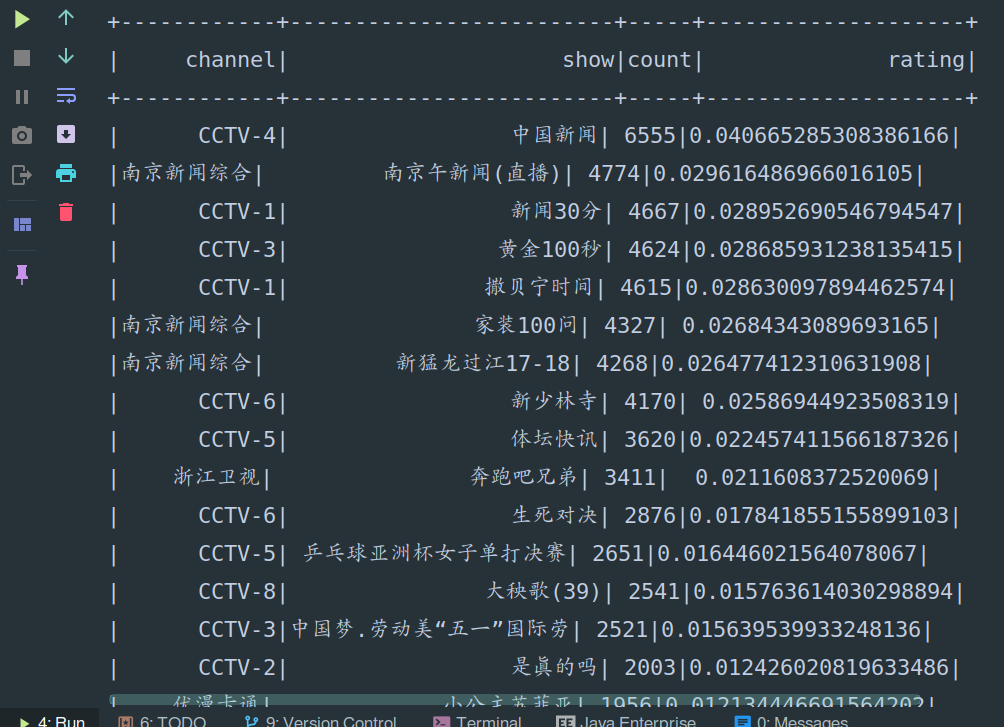
\includegraphics[width=1\linewidth]{rating.png}\\
        ~\\
        图中的count字段代表的是收视人数,rating字段是节目对应的收视率
  \item 用户状态转移图\\
        ~\\
        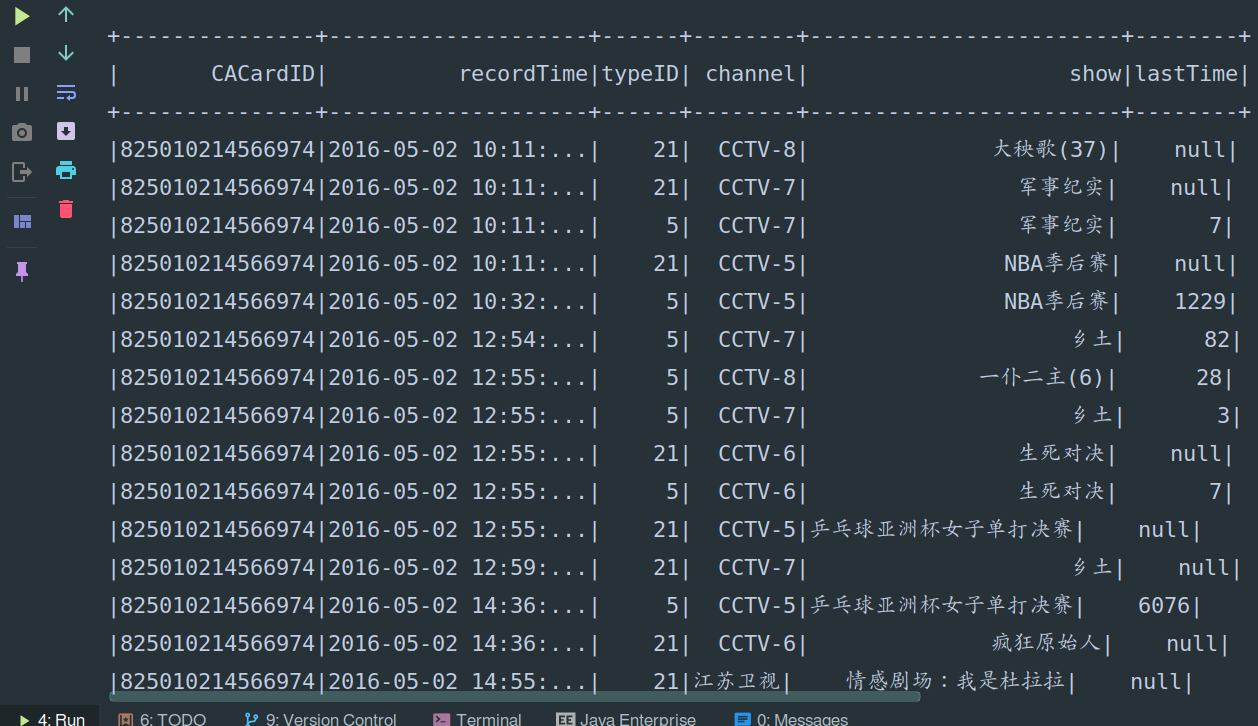
\includegraphics[width=1\linewidth]{transfer.png}\\
        ~\\
        图中的CACardID是同一个用户,而其记录时间在不断的推进,伴随着收视事件(状态)的不断变化和转移,可以看出用户在这段时间内进行的操作和收看节目的变化。
  \item 统计用户收视时间:\\
        ~\\
        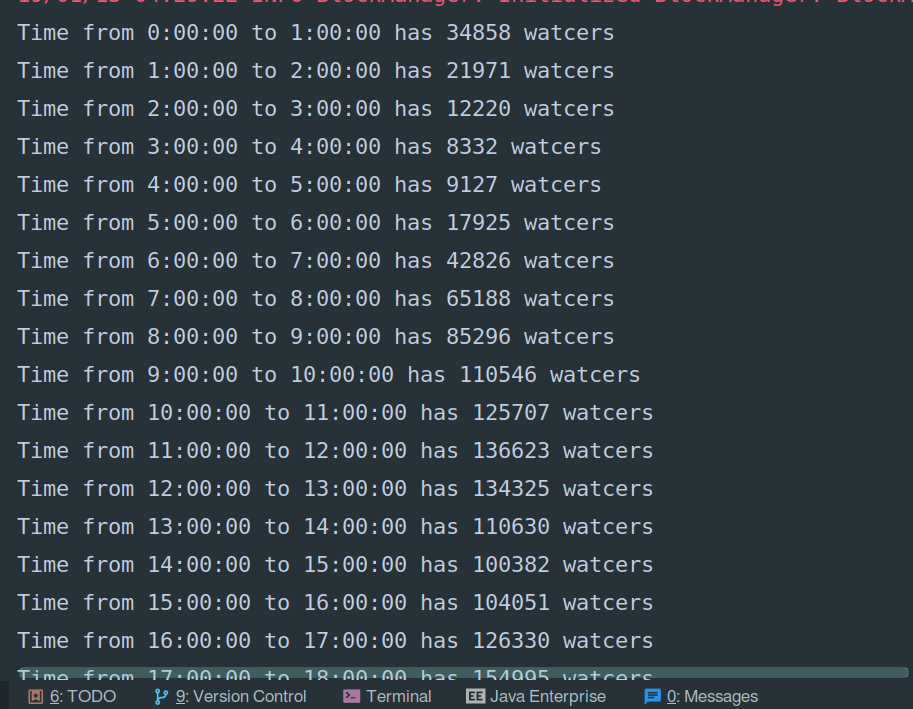
\includegraphics[width=1\linewidth]{watch1.png}\\
        ~\\
        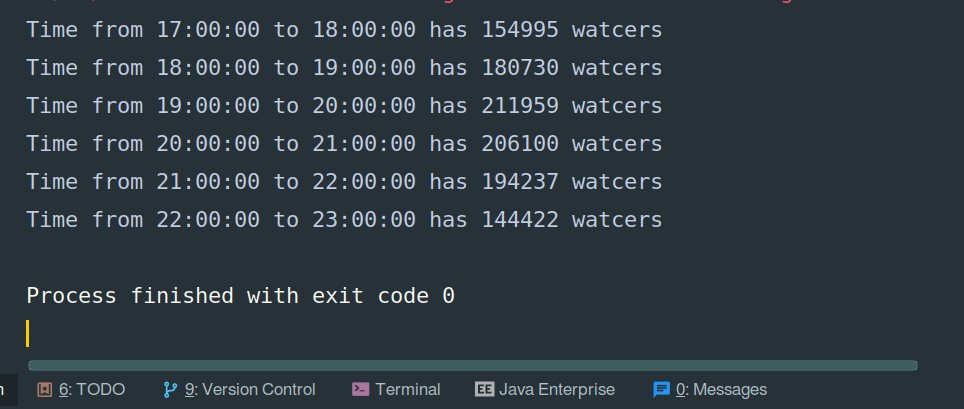
\includegraphics[width=1\linewidth]{watch2.png}\\
        ~\\
        图中显示的是每个时间段内收视的人数\\
        将图中的数据用图表表示出来,可以看到如下的结果:
        横轴代表的是从0点到23点,纵轴代表的是对应时间段的收视人数,第一张图中看出收视最高峰时间在晚上7点钟到晚上8点钟\\
        ~\\
        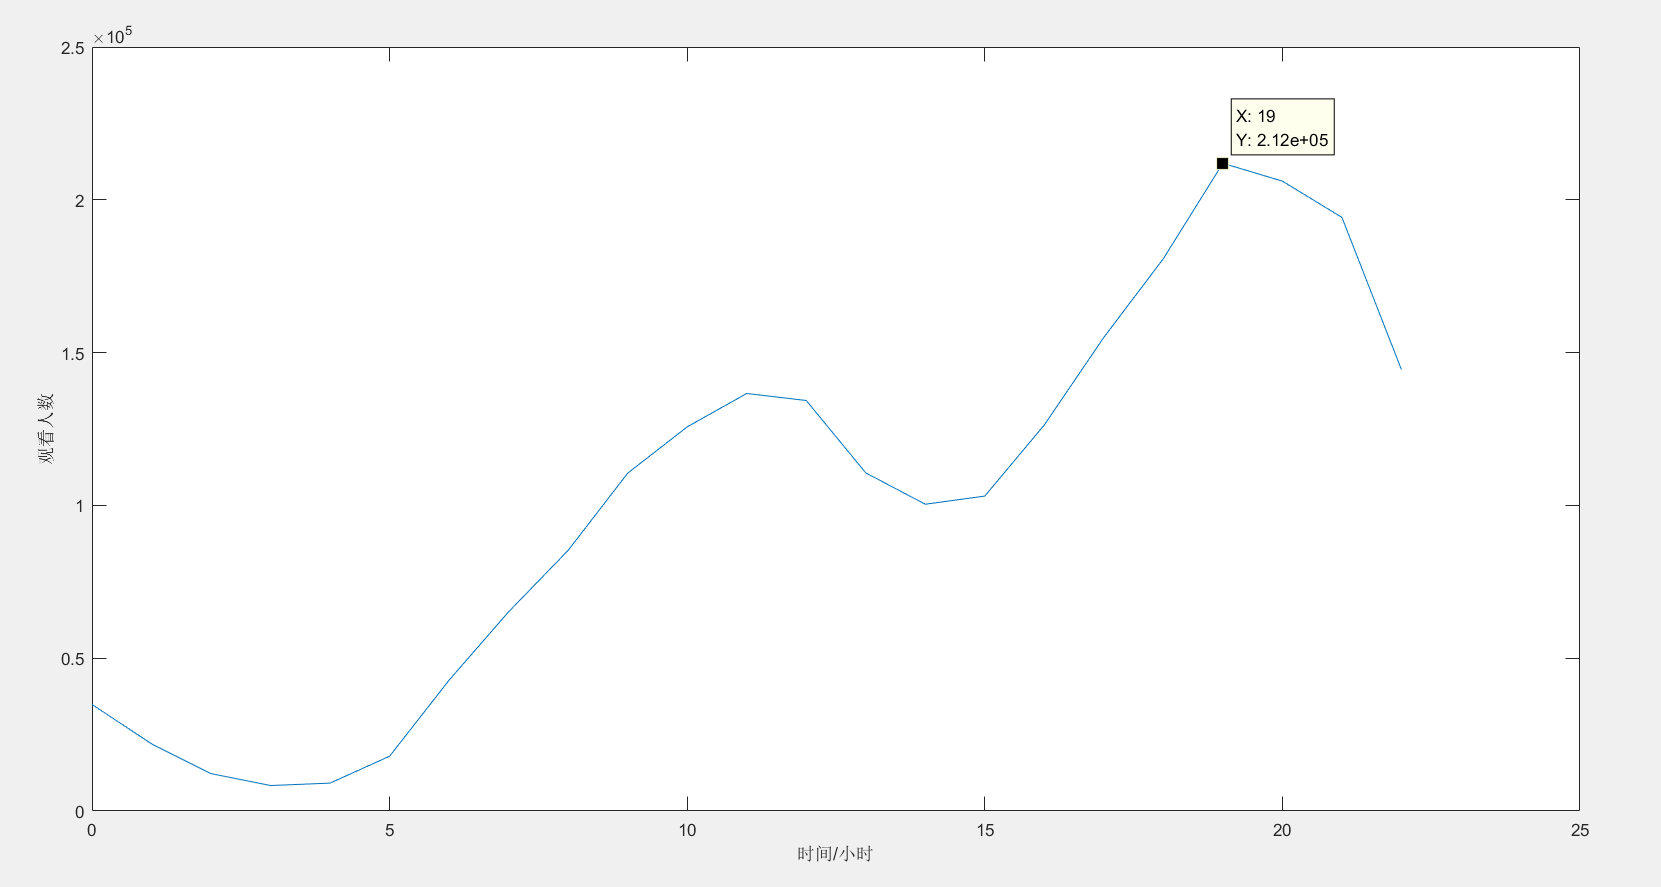
\includegraphics[width=1\linewidth]{plot1.png}\\
        第二张图中看出收视人数最少的时候在凌晨3点钟,次高峰位于中午11点到1点之间\\
        ~\\
        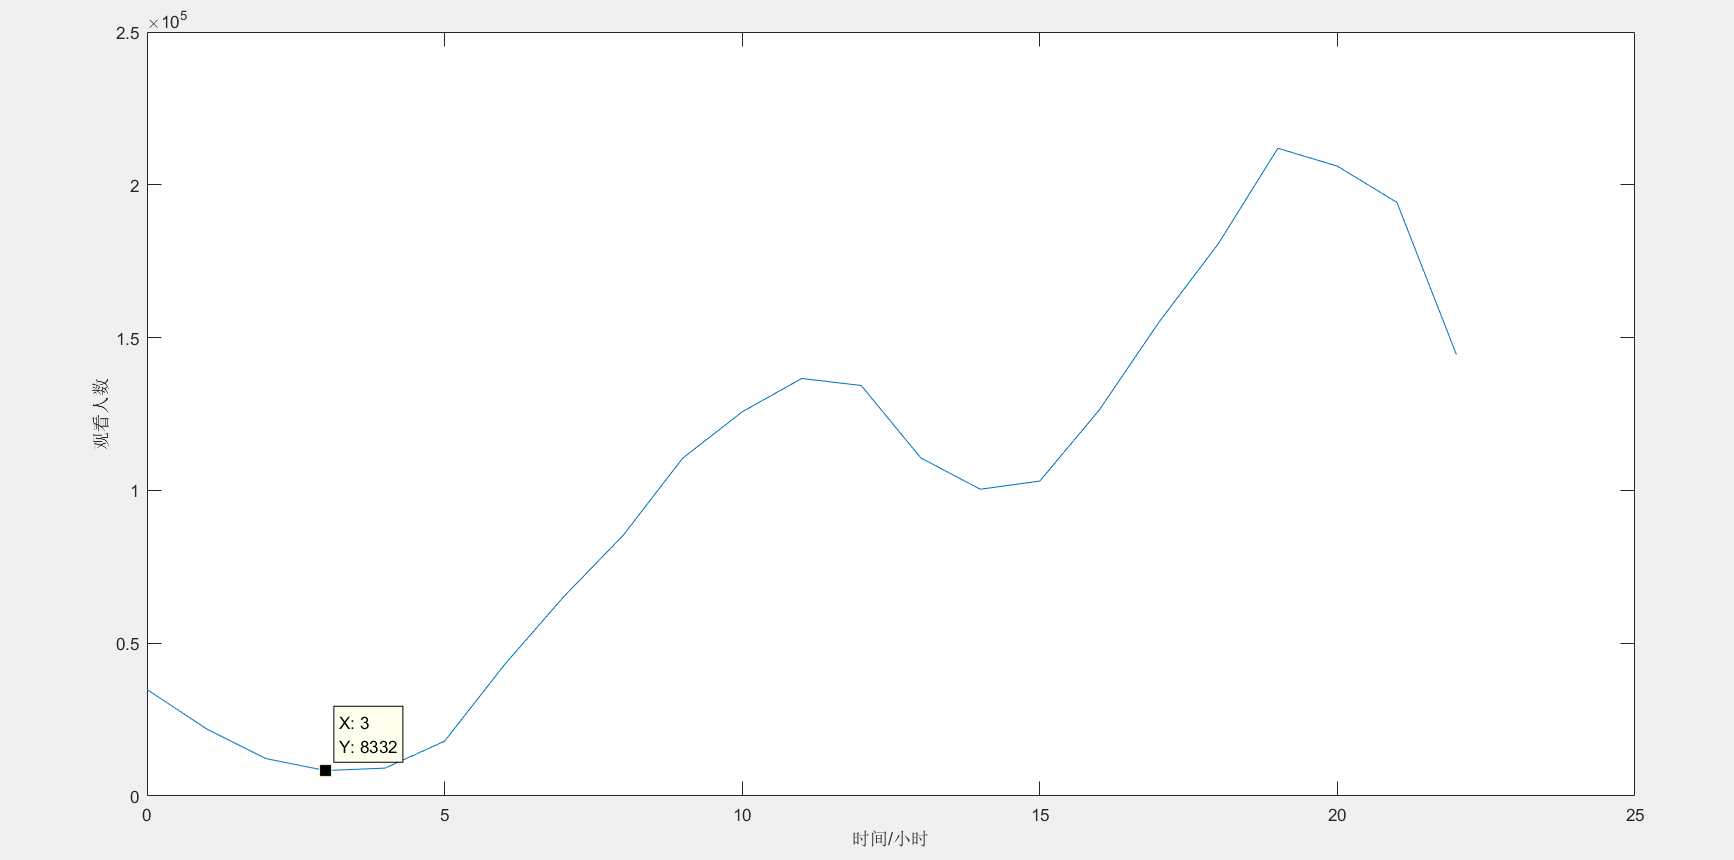
\includegraphics[width=1\linewidth]{plot2.png}\\
        ~\\
  \item 通过回归分析预测节目收视人数\\
        经过准确率和效率的综合考虑,选择随机森林法作为回归分析算法,对节目的收视人数预测结果如下所示:\\
        详细的准确率与效率对比见下一部分的测试环节\\
        ~\\
        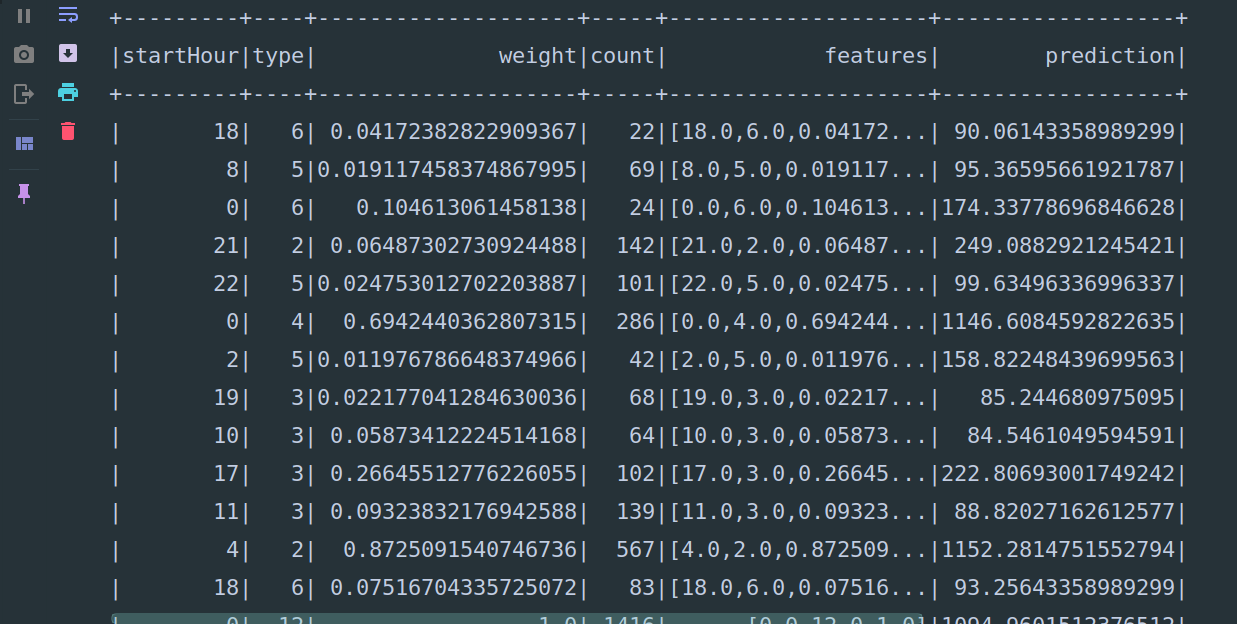
\includegraphics[width=1\linewidth]{prediction31.png}\\
        ~\\
        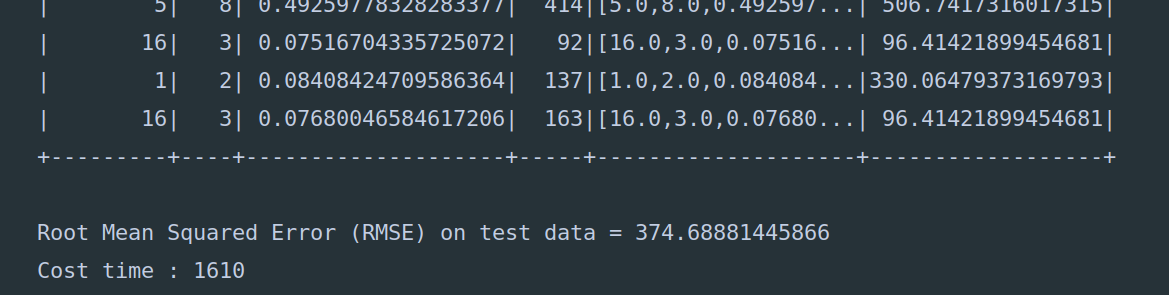
\includegraphics[width=1\linewidth]{prediction32.png}\\
        ~\\
  \item 通过聚类分析为用户推荐节目\\
        第一个图表示了构造的训练集的格式,1~15代表用户收看的对应类型节目的总时长
        第二个图表示了输入一个用户的ID,根据其收视特征进行聚类,然后给用户推荐可能喜爱的节目列表
        ~\\
        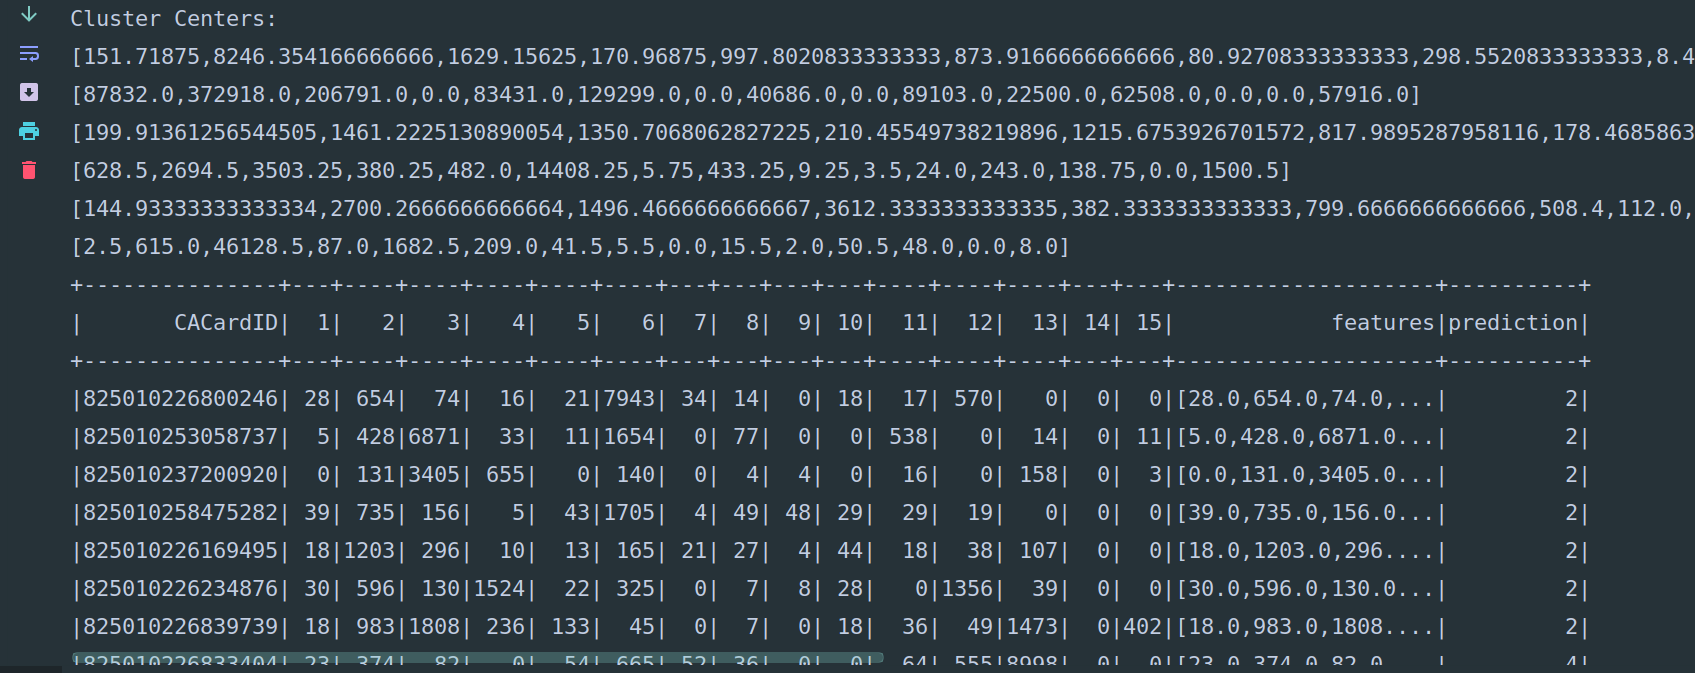
\includegraphics[width=1\linewidth]{cluster.png}\\
        ~\\
        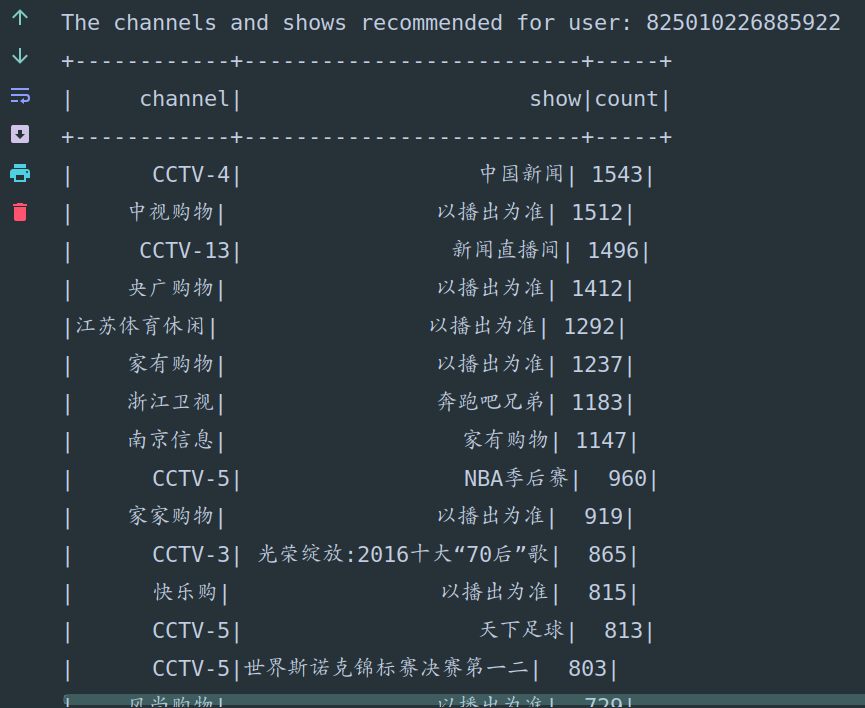
\includegraphics[width=1\linewidth]{recommend.png}\\
\end{itemize}
\section{实验}
\subsection{测试环境}
\begin{flushleft}
  系统:Ubuntu 18.04.1 LTS\\
  CPU:Intel® Core™ i7-6500U CPU @ 2.50GHz × 2 \\
  内存:4.0 GB\\
  磁盘:50GB\\
  网络:本地环回测试\\
\end{flushleft}
\subsection{数据集}
数据集由助教提供,原始大小10GB,我在实验中使用了全部的数据,原始文件由141个较小的文件组成,每个文件是来自一台分布式服务器的数据记录,一行代表一条用户操作记录
\subsection{测试}
由于数据挖掘部分的节目类型这一个维度无法用程序自动获得,需要人工标注,限于时间和人力的因素,训练和测试的规模不能太大,只能小规模抽样实现\\
预测节目的收视人数模型的几种算法的准确率与效率对比:\\
图1.1表示采用的是线性回归的方法,表格中包含了输入特征值,输出特征值count(实际收视人数),prediction是测试集的预测值\\
图1.2表示其误差平均为418人,耗时403ms\\
图2.1表示采用的是决策树的方法,表格中包含了输入特征值,输出特征值count(实际收视人数),prediction是测试集的预测值\\
图2.2表示其误差平均为389人,耗时2633ms\\
图3.1表示采用的是随机森林的方法,表格中包含了输入特征值,输出特征值count(实际收视人数),prediction是测试集的预测值\\
图3.2表示其误差平均为374人,耗时1610ms\\
图4.1表示采用的是梯度提升树的方法,表格中包含了输入特征值,输出特征值count(实际收视人数),prediction是测试集的预测值\\
图4.2表示其误差平均为384人,耗时42s\\
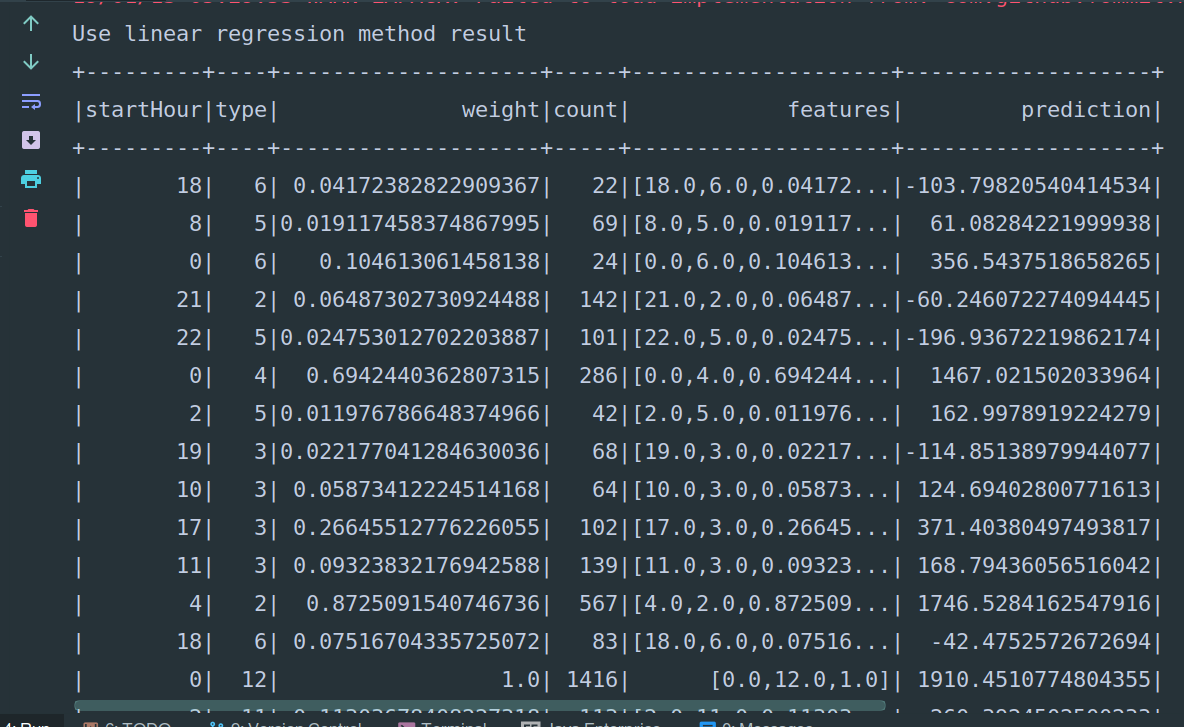
\includegraphics[width=1\linewidth]{prediction11.png}\\
图1.1\\
~\\
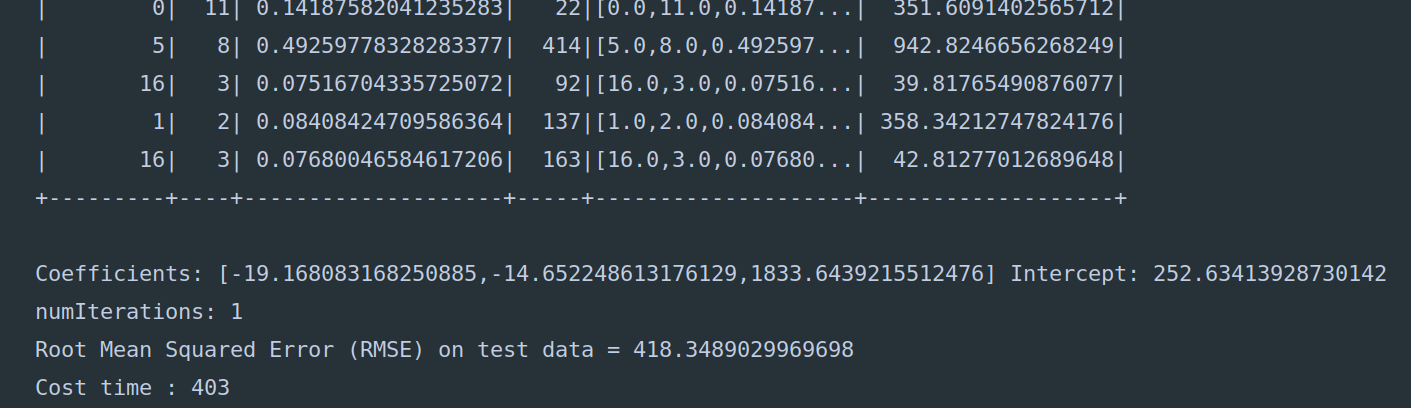
\includegraphics[width=1\linewidth]{prediction12.png}\\
图1.2\\
~\\
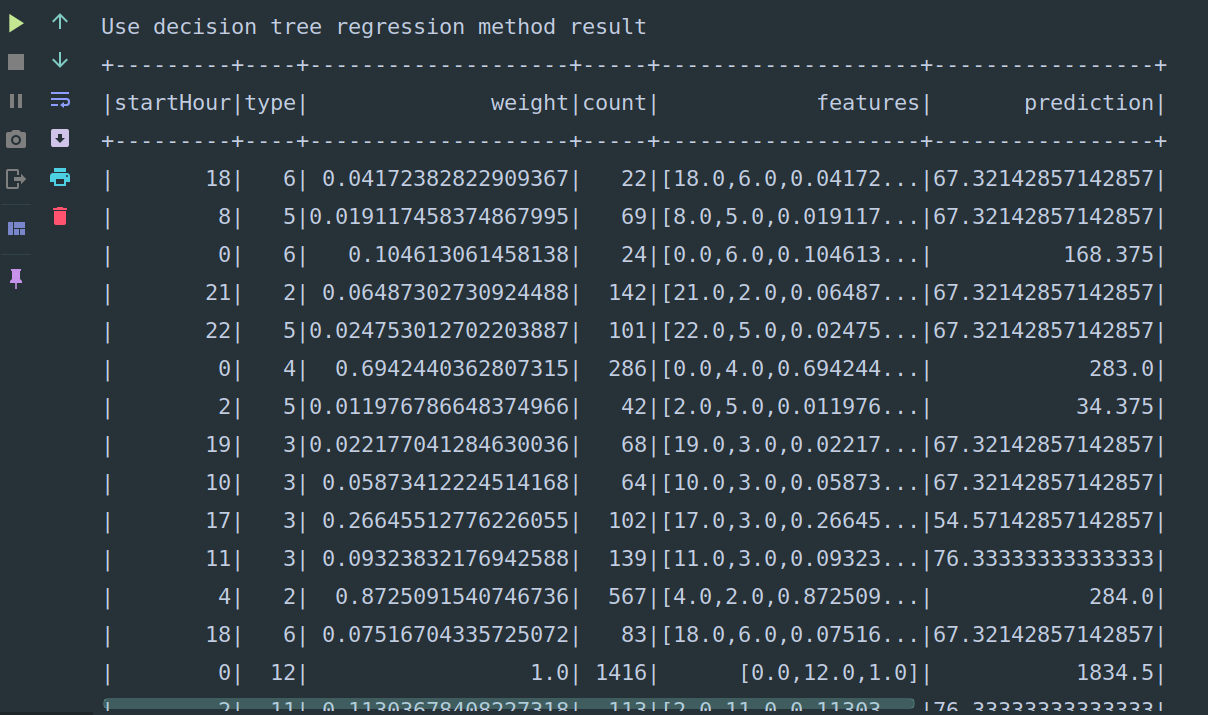
\includegraphics[width=1\linewidth]{prediction21.png}\\
图2.1\\
~\\
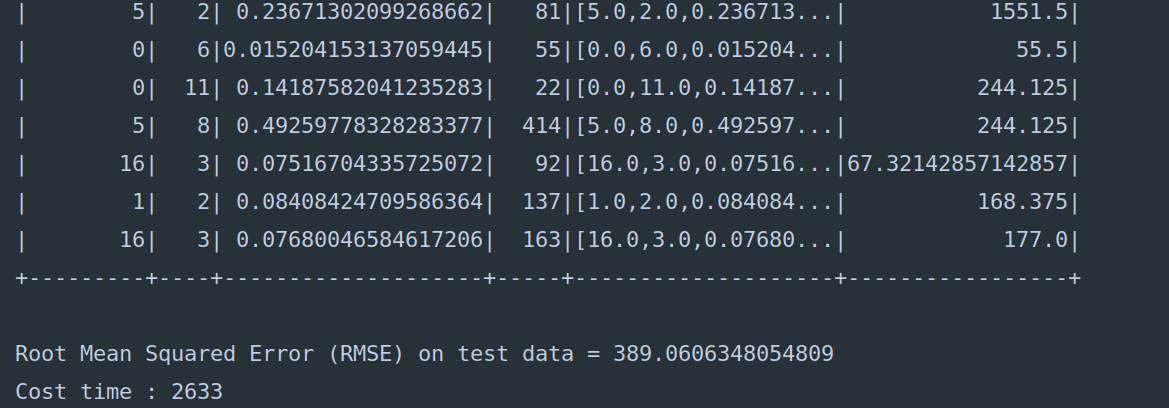
\includegraphics[width=1\linewidth]{prediction22.png}\\
图2.2\\
~\\
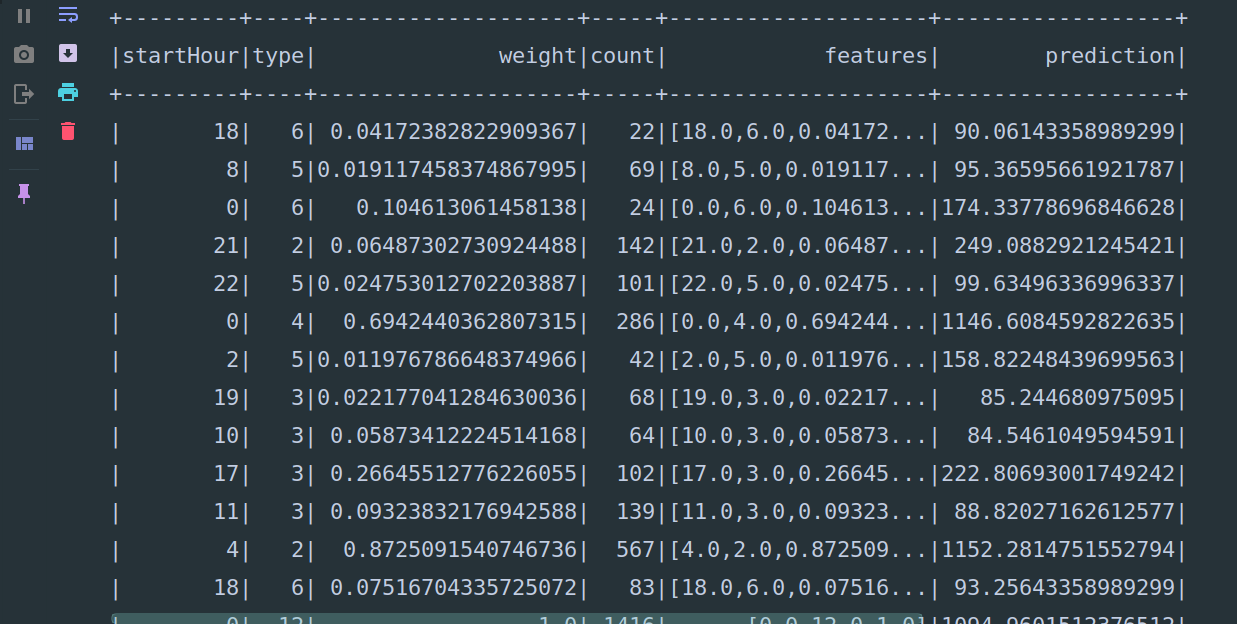
\includegraphics[width=1\linewidth]{prediction31.png}\\
图3.1\\
~\\
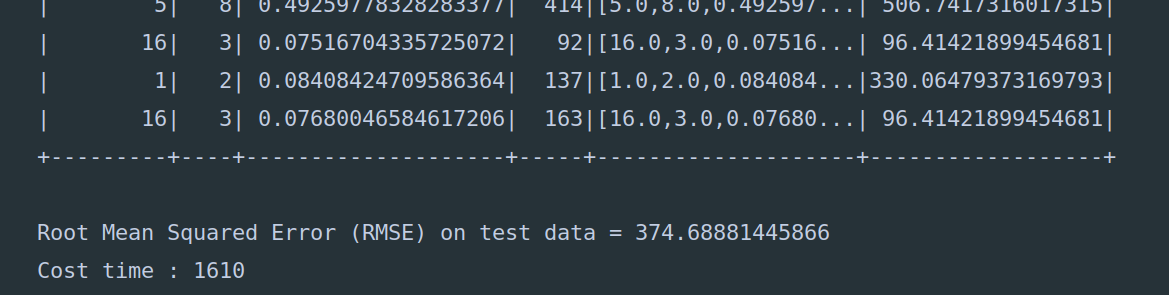
\includegraphics[width=1\linewidth]{prediction32.png}\\
图3.2\\
~\\
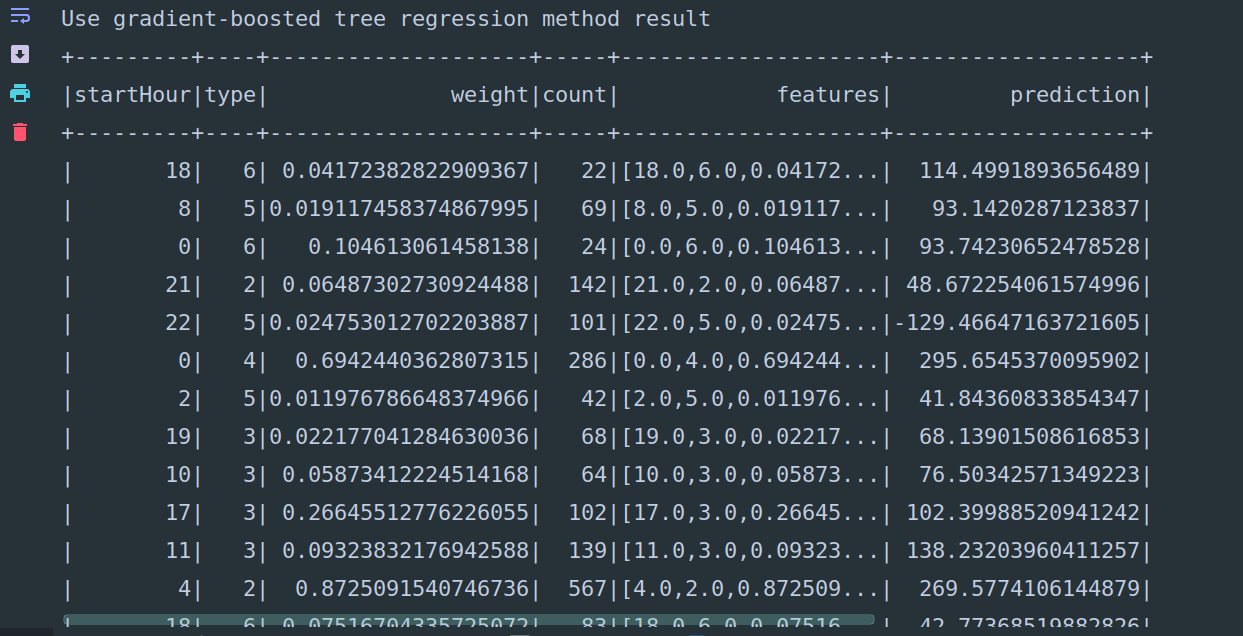
\includegraphics[width=1\linewidth]{prediction41.png}\\
图4.1\\
~\\
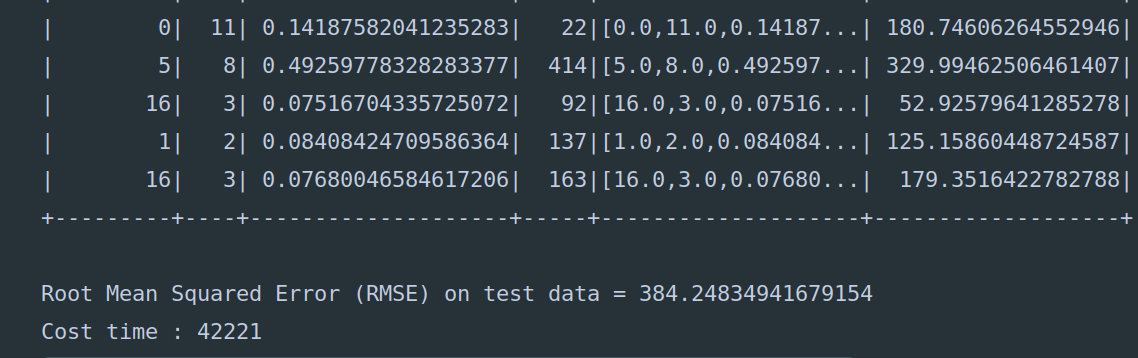
\includegraphics[width=1\linewidth]{prediction42.png}\\
图4.2\\
~\\
\section{结论}
\begin{itemize}
  \item Spark的内存处理框架可以处理内存无法容纳的数据量,并且具有良好的可扩展性。其内存运行模式在机器学习模型的训练过程中,效率较高,能够满足对时间的要求
  \item 在对收视时间的统计中,发现在一天中的凌晨3点钟到4点钟时间段,收视人数最少,在晚上7点钟时的收视人数最多,中午和晚上都是收视的高峰期
  \item 在回归分析中,在对离散数据的拟合时,决策树及基于决策树的随机森林和梯度上升树都具有较高的准确度,其准确度远远高于线性回归。同时在效率方面,随机森林算法的效率最高,但是与决策树和线性回归算法相差不大,梯度上升树算法的效率最低,其运行时间达到了决策树算法的30倍以上。综合准确率和算法效率的综合考虑,应该选择随机森林算法作为回归模型的回归算法。
  \item 对用户的收视喜好进行聚类分析能够对用户进行有效的分类,并能够用于对用户收视节目的推荐与预测
\end{itemize}
\end{document}
